A test was carried out to study the influence of the fiber diameter in the tritium measurement. To do so, a simulation, for a single scintillating fiber $20~\cm$ length and two different diameters, $1~\mm$ and $2~\mm$ (the commercial options given by Saint-Gobain), were compared.

An important point is how the fiber diameter affect to cosmic ray detection, which is an important component of the background of the TRITIUM monitor. The energy deposited in the scintillating fiber by a cosmic ray event is proportional to the active volume crossed, which is larger for $2~\mm$ fibers. Therefore, the cosmic ray signal obtained for a measured cosmic event will be larger for a detector based on $2~\mm$ diameter. The objective of this study is to find the design with which a lower background is obtained in the region of interest of tritium detection, ROI (up to $18~\keV$).

For this test, the tritiated water source was replaced by a cosmic ray source, generated by the CRY library\footnote{CRY library, Cosmic-Ray Shower library} \cite{CRYwebsite}, \cite{CRYpaper}. The CRY library is a package based on objected-oriented technology and implemented in the C++ programming language. This library is used to generate cosmic-ray shower distributions for different particles (muons, neutrons, protons, electrons, photons and pions). The cosmic source shape used in this simulation is a horizontal square of $1 \times 1~\meter ^2$ located at a height of $35~\cm$ (above the detector) with the typical distribution of cosmic particles at see level. 

The distribution of energy deposited in scintillating fibers by cosmic ray events are shown in Figure \ref{fig:DiameterComparison} for both cases, $1~\mm$ and $2~\mm$ fibers.

\begin{figure}[hbtp]
\centering
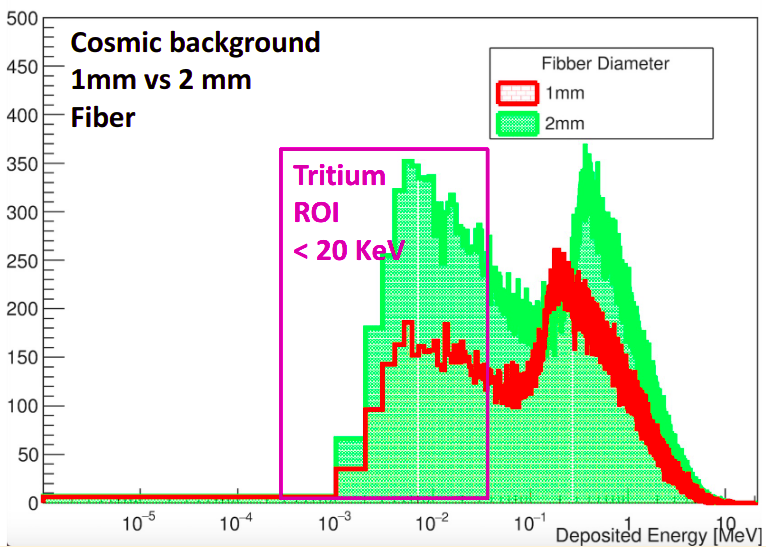
\includegraphics[scale=0.4]{Figures/8SimulationsResults/81TRITIUMDesign/814Diameter/ComparisonDiameter.png}
\caption{Comparison of the energy deposition of cosmic ray events in scintillating fibers of $1~\mm$ and $2~\mm$ in diameter.\label{fig:DiameterComparison}}
\end{figure}

As can be seen in the figure, a smaller background is measured for fiber diameters of $1~\mm$, which reduces the low detection level LDL of the detector. There are other reasons that favor the use of $2~\mm$ fibers, such us their greater resistance and an improvement to the passage of water through them, so a experimental test is needed to choose the best design.